\section{Requirements}

\subsection{Overall Requirements Specification}
\subsubsection{Problem Statement}
In the table \ref{table:problem-statement}, the finished problem, the problem statement and related questions are listed.
\begin{table}[ht]
    \begin{tabularx}{\textwidth}{|>{\RaggedRight}p{4cm}|>{\RaggedRight}X|}
        \hline
        \textbf{Problem} & The current production line is not efficient enough to keep up with the demand of the beer, while still maintaining a quality product\\
        \hline
        \textbf{Problem Statement} & How to control and optimise the brewing machine, to maximise the production of high quality beer\\
        \hline
        \textbf{Related questions} & 
            \begin{itemize}
                \item How can we optimise the production?
                \item How can we utilise calculus and linear algebra to provide a meaningful overview of the production line, based on statistics?
                \item How can we create a web based front end for the MES?
                \item How can we separate the different aspects of the system (separation of concerns)
            \end{itemize}
        \\ 
        \hline
    \end{tabularx}
    \caption{Problem statement showcase} 
    \label{table:problem-statement}
\end{table} 

\subsubsection{Summary of requirements}
The group's proposed solution will adhere to the requirements given by the brewery Refslevbæk Bryghus A/S.

The manufacturing execution system, MES, must be able to control the brewery’s production.
It must be able to start and stop the production line,
as well as monitor the production and collect data from the production line.
The data must be stored for further analysis.
The MES must be able to keep track of the batches that the new machine is producing,
as well as collect various data from the machine that is associated with the current batch number.
After a finished batch production, the MES must be able to produce a batch report.
The report must contain the following.

\begin{itemize}
    \item This Batch ID
    \item Product type
    \item Amount of products (total, defect and acceptable)
    \item Amount of time used in the different states
    \item Logging of temperature over the production time
    \item Logging of humidity over the production time
\end{itemize}

The MES/SCADA (Supervisory control and data acquisition) system must be able to monitor the production and display live relevant data from the machine.
The documentation of the system must contain an illustration that defines the different components in the setup, in relation to the ISA88\^{}1213 Part 1 Physical Hierarchy model.
The system must have a visualisation that can be accessed and used to display production data.
The system must be able to collect the necessary data from the machine and calculate the overall equipment effectiveness, OEE\^{}131516, of the machine. The OEE must be available to be displayed by the system.
The system must be able to estimate the error function associated with the different products.
The system must be able to find the optimal production speed for each product type, based on an error simulation and the appertaining graph upon which the error simulation is built.

\subsubsection{List of requirements}
Below is a list of the above requirements. These requirements have been
prioritised using the MoSCoW method, where M is for Must have, S is for
Should have, C is for could have, and W is for Won't have. 

\begin{table}[H]
    \begin{tabularx}{\textwidth}{|>{\RaggedRight}p{1cm}|>{\RaggedRight}p{4cm}|>{\RaggedRight}X|>{\RaggedRight}p{1cm}|}
        \hline
        \textbf{ID} & \textbf{Name} & \textbf{Description} & \textbf{Prio} \\
        \hline
        R01 & Control production line & Control the brewery's production & M \\
        \hline
        R02 & Control production line & Start/stop production line & M \\
        \hline
        R03 & Monitor production & Monitor data from the production line & M \\
        \hline
        R04 & Monitor production & Store the collected data for further analysis & M \\
        \hline
        R05 & Administer batches & Keep track of produced batches (batch ID) & M \\
        \hline
        R06 & Store batch info & Collect various data associated with current batch number from the machine & M \\
        \hline
        R07 & Batch report & Produce a batch report (PDF/dashboard style format) & M \\
        \hline
        R08 & Live data & Monitor and display live relevant data from the machine & M \\
        \hline
        R09 & Documentation & Documentation must contain an illustration that defines the different components in the setup in relation to the ISA88\^{}1213 Part 1 Physical Hierarchy model & M \\
        \hline
        R10 & Visualisation & Visualisation that can be accessed and used to display the production data & M \\
        \hline
        R11 & OEE & Collect necessary data from the machine and calculate the OEE. OEE must be available to be displayed by the system & M \\
        \hline
        R12 & Estimate error function & Estimate the error function associated with the products & S \\
        \hline
        R13 & Optimal Production speed & Estimate the optimal production speed for each product type & M \\
        \hline
    \end{tabularx}
    \caption{List of requirements} 
    \label{table:Requirements}
\end{table}

\subsection{Selected Detailed Requirements}

\subsubsection{Functional \& Non-Functional Requirements}
In table \ref{table:sup_requirements} you can see a description of Functional and
Non-Functional requirements. 
FURPS+ is a model for classifying functional and non-functional requirements.
The acronym stands for functionality, usability, reliability, performance, and supportability.
The '+' sign stands for design constraints, implementation requirements,
interface requirements, and physical requirements.


\begin{table}[ht]
    \begin{tabularx}{\textwidth}{|>{\RaggedRight}p{3.3cm}|>{\RaggedRight}p{0.6cm}|>{\RaggedRight}X|}
        \hline
        \textbf{FURPS+}  & \textbf{\#} & \textbf{Demands} \\
        \hline
        Functionality  	& S01 & Improve the beer machine by increasing quantity while maintaining quality \\
        \hline
        Usability      	& S02 & Documentation on usage of the REST API \\
        \hline
        Reliability    	& S03 & On server reboot, the application will automatically restart \\
        \hline
        Performance    	& S04 & Max response time (API: 400 ms) \\
        \hline
        Supportability 	& S05 & Minimum browser versions (JavaScript version 6)\\
        \hline
        Design constraints 	& S06 & Na \\
        \hline
        \multirow{5}{100}{Implementation requirements} & S08 & Should be controlled via MES\\
        \cline{2-3}
                & S08 & MES should be able to keep track of Batches\\
        \cline{2-3}
                & S09 & Monitor production (Live data)\\
        \cline{2-3}
                & S10 & Estimate error function\\
        \cline{2-3}
                & S11 & Optimal production speed\\
        \hline
        \multirow{14}{100}{Interface requirements } & S12 & Show OEE \\
        \cline{2-3}
                & S13 & Show Batch Report that include:
            \begin{itemize}
                \item Batch ID
                \item Product type
                \item Amount of products (total, defect and acceptable)
                \item Amount of time used in the different states
                \item Logging of temperature over the production time
                \item Logging of humidity over the production time
            \end{itemize} \\
        \cline{2-3}
            & S14 & Visualisation \\
        \hline
        Physical requirements & S14 & The group should work with the beer 
        production machine provied by SDU \\
        \hline
    \end{tabularx}
    \caption{Supplementary Requirements} 
    \label{table:sup_requirements}
\end{table} 

\subsubsection{The Physical Setup (The Brewery Machine)}

The machine can produce different kinds of beer depending on the recipe
used. The beer is produced in batches which have their own batch id. When 
producing a batch the recipe, quantity, speed and batch id can be configured by 
an external system. When a batch has been produced the quality inspection system 
measures the quality for future use. These values are accessible in the machines 
SCADA system. The SCADA system monitors and supervises both the machines PLC 
system and the internal sensors PLC system as well as the quality inspection 
system.

\myparagraph{Sensors}
To ensure the most optimal environment beer production the 
machine is equipped with three sensors that measure the environment while 
production is happening. This data is useful as it gives insight into the 
internal environment of the machine while producing products. Currently, it 
measures temperature, humidity and vibration. The machine itself is not able to 
collect these data and are collected by an external system.

\myparagraph{Quality Inspection System}
To make it possible to calculate an error function, the system is 
equipped with a sophisticated quality inspection system. This system is key to 
optimising the production by giving data about the different error functions of 
the configurations so that they can be configured otherwise to maximise 
production. Each produced product is inspected and if the quality is low enough
the product will fail. When a batch is finished the QIS will output the amount 
of failed and passed products. The result is then used to calculate the error
function.


\subsubsection{The Simulator}
The group is going to use the simulator software to test the software during the
development cycle.
It is important to note that the simulator is not a replacement of the machine
since there is only so much randomness and correctness you can get from a 
simulator. 
It is still very important to have the simulator, when making prototypes and 
performing multiple tests on it, so any regressions won't be pushed to 
the production system(the beer machine).

\subsection{Use Cases}
Use cases are written descriptions of how a user will perform different tasks
on a system. They outline a systems behaviour as it responds to a request from
the user. Each use case is represented as a sequence of steps, beginning with
the users goal and ending when it that goal is fulfilled. \\

The first step in developing use cases is to determine the actors.


% \begin{table}[ht]
%    \begin{tabularx}{\textwidth}{|>{\RaggedRight}p{3cm}|>{\RaggedRight}X|>{\RaggedRight}p{2.5cm}|}
%     \hline
%     \textbf{Use Case ID}   & \textbf{Name}                                 & \textbf{Definition}\\ \hline
%     UC01                   & Start production line                         & User \\ \hline
%     UC02                   & Stop production line                          & User \\ \hline
%     UC03                   & Monitor and store data from production line   & SCADA \\ \hline
%     UC04                   & Monitor and display relevant data live        & SCADA \\ \hline
%     UC05                   & Create batch report                           & MES \\ \hline
%     UC06                   & Calculate OEE                                 & MES \\ \hline
%     UC07                   & Estimate the error function                   & MES \\ \hline
%     UC08                   & Find optimal production speed                 & MES \\ \hline
%     \end{tabularx}
%     \caption{Use Cases}
%     \label{table:use_cases}
%     \end{table}

\subsubsection{Actor List}
In order to determine who will be able to access the system, the actors are
found. An actor is defined as any external system or user that communicates
with the system. Not every actor can necessarily be found at the given time,
meaning other actors may be found later during development.

The identified actors can be seen in table \ref{table:actor_list}. With these
actors, a visualisation can be made, depicting how the different actors
communicate with the system.

\begin{table}[ht]
     \begin{tabularx}{\textwidth}{|>{\RaggedRight}p{2.5cm}|>{\RaggedRight}p{8cm}|>{\RaggedRight}X|}
     \hline
     \textbf{Actor} 				& \textbf{Description}                                                                                                              				& \textbf{Goal} \\ \hline
     \multirow{2}{*}{User (p)}      & The user represents the worker of the machine. The user will use the control panel to control the machine.                                  		& 	\begin{itemize}
     																																														\item Control machine
     																																														\item Start new batches
     																																													\end{itemize} \\ \hline
     \multirow{2}{*}{BPM (s)}     	& The beer production machine is responsible for supplying data to the MES and producing the beer.       											& \begin{itemize} 
     																																														\item Collect and save data
     																																														\item Communicate between hardware and MES 
     																																									 				\end{itemize} \\ \hline
    \end{tabularx}
    \caption{Actor list}
    \label{table:actor_list}
\end{table}

\subsubsection{Detailed Use Cases}
When the actors have been determined, use cases can be developed. These use
cases add value because they help explain how the system behaves and which
functions to include when developing the system. As seen below, in table
\ref{table:usecase_start}, which represents the sequence of steps happening
when a user wants to start the beer production machine. This use case clarifies
the functions needed to fulfil the users goal, to start the production machine.

% start production
\begin{table}[ht]
    \begin{tabularx}{\textwidth}{|>{\RaggedRight}X|}
        \hline
        \textbf{ID:} UC01  \\
        \hline
        \textbf{Primary actor:} The user \\
        \hline
        \textbf{Secondary actor:} Beer production machine \\
        \hline
        \textbf{Short description:} The MES must be able to start the brewery's
        production \\
        \hline
        \textbf{Pre conditions:} The beer production machine needs to be in
        ready mode, that is, not producing beer. \\
        \hline
        \textbf{Main flow:} \\
        	1. This use case starts when a user wants to start the beer
        	production machine. \\
        	2. The user chooses what kind of beer to be produced. \\
        	3. The user sets production speed. \\
        	4. The user sets batch id. \\
        	5. The user sets amount of beers to be produced. \\
        	6. The user presses the start button. \\
        	7. The MES starts the machine. \\
        	8. When the production has finished, the MES stores data from the
        	production. \\

		\hline
        \textbf{post conditions:} The beer production machine is turned on \\
        \hline
        \textbf{Alternative flow:} \\
        	Step 8: If the machine does not complete the production (for various
        	reasons) the production stops and stores the data from the machine
        	and the user receives an error message. \\
        \hline
    \end{tabularx}
    \caption{Production Control: Start machine}
    \label{table:usecase_start}
\end{table}

%% BELOW USE CASES BELONGS IN APPENDIX, IF PAGENUMBERS ALLOW IT
% % stop production
% \begin{table}[ht]
%     \begin{tabularx}{\textwidth}{|>{\RaggedRight}X|}
%         \hline
%         \textbf{ID:} UC02  \\
%         \hline
%         \textbf{Primary actor:} The user \\
%         \hline
%         \textbf{Secondary actor:} Beer production machine \\
%         \hline
%         \textbf{Short description:} The MES must be able to stop the brewery's
%         production \\
%         \hline
%         \textbf{Pre conditions:} The beer production machine needs to be on \\
%         \hline
%         \textbf{Main flow:} \\
%         	1. This use case starts when a user wants to shut down the beer
%         	production machine. \\
% 			2. The user presses the stop button \\
% 			3. The MES stores the data from the beer production machine \\
% 			4. The beer production machine stops \\
% 		\hline
%         \textbf{post conditions:} The beer production machine is turned off \\
%         \hline
%         \textbf{Alternative flow:} \\
%         \hline
%     \end{tabularx}
%     \caption{Production Control: Stop production} 
%     \label{table:usecase_stop}
% \end{table}

% % abort
% \begin{table}[ht]
%     \begin{tabularx}{\textwidth}{|>{\RaggedRight}X|}
%         \hline
%         \textbf{ID:} UC03  \\
%         \hline
%         \textbf{Primary actor:} The user \\
%         \hline
%         \textbf{Secondary actor:} Beer production machine \\
%         \hline
%         \textbf{Short description:} The MES must be able to abort the current
%         production. \\
%         \hline
%         \textbf{Pre conditions:} The production needs to be on and producing
%         beer. \\
%         \hline
%         \textbf{Main flow:} \\
%         	1. This use case starts when a user wants to abort the current
%         	production. \\
%         	2. The user presses the abort button \\
% 			3. The MES stores the data from the beer production machine \\
% 			4. The beer production machine aborts \\
% 		\hline
%         \textbf{post conditions:} The beer production machine aborted the
%         current production \\
%         \hline
%         \textbf{Alternative flow:} \\
%         \hline
%     \end{tabularx}
%     \caption{Production Control: Abort the current production} 
%     \label{table:usecase_abort}
% \end{table}

% % reset
% \begin{table}[ht]
%     \begin{tabularx}{\textwidth}{|>{\RaggedRight}X|}
%         \hline
%         \textbf{ID:} UC04  \\
%         \hline
%         \textbf{Primary actor:} The user \\
%         \hline
%         \textbf{Secondary actor:} Beer production machine \\
%         \hline
%         \textbf{Short description:} The MES must be able to reset the beer
%         production machine. \\
%         \hline
%         \textbf{Pre conditions:} The beer production machine needs to be in
%         ready mode, that is, not producing beer. \\
%         \hline
%         \textbf{Main flow:} \\
%         	1. This use case starts when a user wants to reset the beer
%         	production machine \\
%         	2. The user presses the reset button \\
% 			3. The beer production machine resets \\
% 		\hline
%         \textbf{post conditions:} The beer production machine has been reset \\
%         \hline
%         \textbf{Alternative flow:} \\
%         \hline
%     \end{tabularx}
%     \caption{Production control: Reset the machine}
%     \label{table:usecase_reset}
% \end{table}

% % clear
% \begin{table}[ht]
%     \begin{tabularx}{\textwidth}{|>{\RaggedRight}X|}
%         \hline
%         \textbf{ID:} UC05  \\
%         \hline
%         \textbf{Primary actor:} The user \\
%         \hline
%         \textbf{Secondary actor:} The beer production machine \\
%         \hline
%         \textbf{Short description:} The MES must be able to clear the beer
%         production machine. \\
%         \hline
%         \textbf{Pre conditions:} The beer production machine needs to be in
%         ready mode, that is, not producing beer. \\
%         \hline
%         \textbf{Main flow:} \\
%         	1. This use case starts when a user wants to clear the beer
%         	production machine \\
%         	2. The user presses the clear button \\
% 			3. The beer production machine clears \\
% 		\hline
%         \textbf{post conditions:} The beer production machine has been cleared \\
%         \hline
%         \textbf{Alternative flow:} \\
%         \hline
%     \end{tabularx}
%     \caption{Production control: Clear the machine}
%     \label{table:usecase_clear}
% \end{table}

% % display live data
% \begin{table}[ht]
%     \begin{tabularx}{\textwidth}{|>{\RaggedRight}X|}
%         \hline
%         \textbf{ID:} UC06  \\
%         \hline
%         \textbf{Primary actor:} The user \\
%         \hline
%         \textbf{Secondary actor:} The beer production machine \\
%         \hline
%         \textbf{Short description:} The MES needs to display live data from the
%         production. \\
%         \hline
%         \textbf{Pre conditions:} The beer production machine needs to be on and
%         producing beer. \\
%         \hline
%         \textbf{Main flow:} \\
%         	1. This use case starts when the user wants to see data from the
%         	production. \\
% 			2. The MES collects the necessary data from the beer production
% 			machine. \\
% 			3. The MES displays the relevant data for the user. \\
% 		\hline
%         \textbf{post conditions:} Live data has been displayed for the user. \\
%         \hline
%         \textbf{Alternative flow:} \\
%         \hline
%     \end{tabularx}
%     \caption{Production monitoring: Display live data}
%     \label{table:usecase_displayLiveData}
% \end{table}

% % generate batch report
% \begin{table}[ht]
%     \begin{tabularx}{\textwidth}{|>{\RaggedRight}X|}
%         \hline
%         \textbf{ID:} UC07  \\
%         \hline
%         \textbf{Primary actor:} The user \\
%         \hline
%         \textbf{Secondary actor:} The beer production machine \\
%         \hline
%         \textbf{Short description:} The MES needs to be able to generate a batch
%         report from previous batches. \\
%         \hline
%         \textbf{Pre conditions:} The beer production machine needs to have
%         produced a batch. \\
%         \hline
%         \textbf{Main flow:} \\
%         	1. This use case starts when the user wants to see a batch report
%         	from previous productions. \\
% 			2. The MES generates a batch report \\
% 			3. The MES displays the batch report to the user. \\
% 		\hline
%         \textbf{post conditions:} A batch report has been displayed for the
%         user. \\
%         \hline
%         \textbf{Alternative flow:} \\
%         \hline
%     \end{tabularx}
%     \caption{Batch report: Generate batch report}
%     \label{table:usecase_batchReport}
% \end{table}

\subsubsection{Use Case Diagram}
Below, in figure \ref{figure:ucdiagram}, an overview of the use cases for the
MES can be seen.

\begin{figure}[ht]
	\centering 
	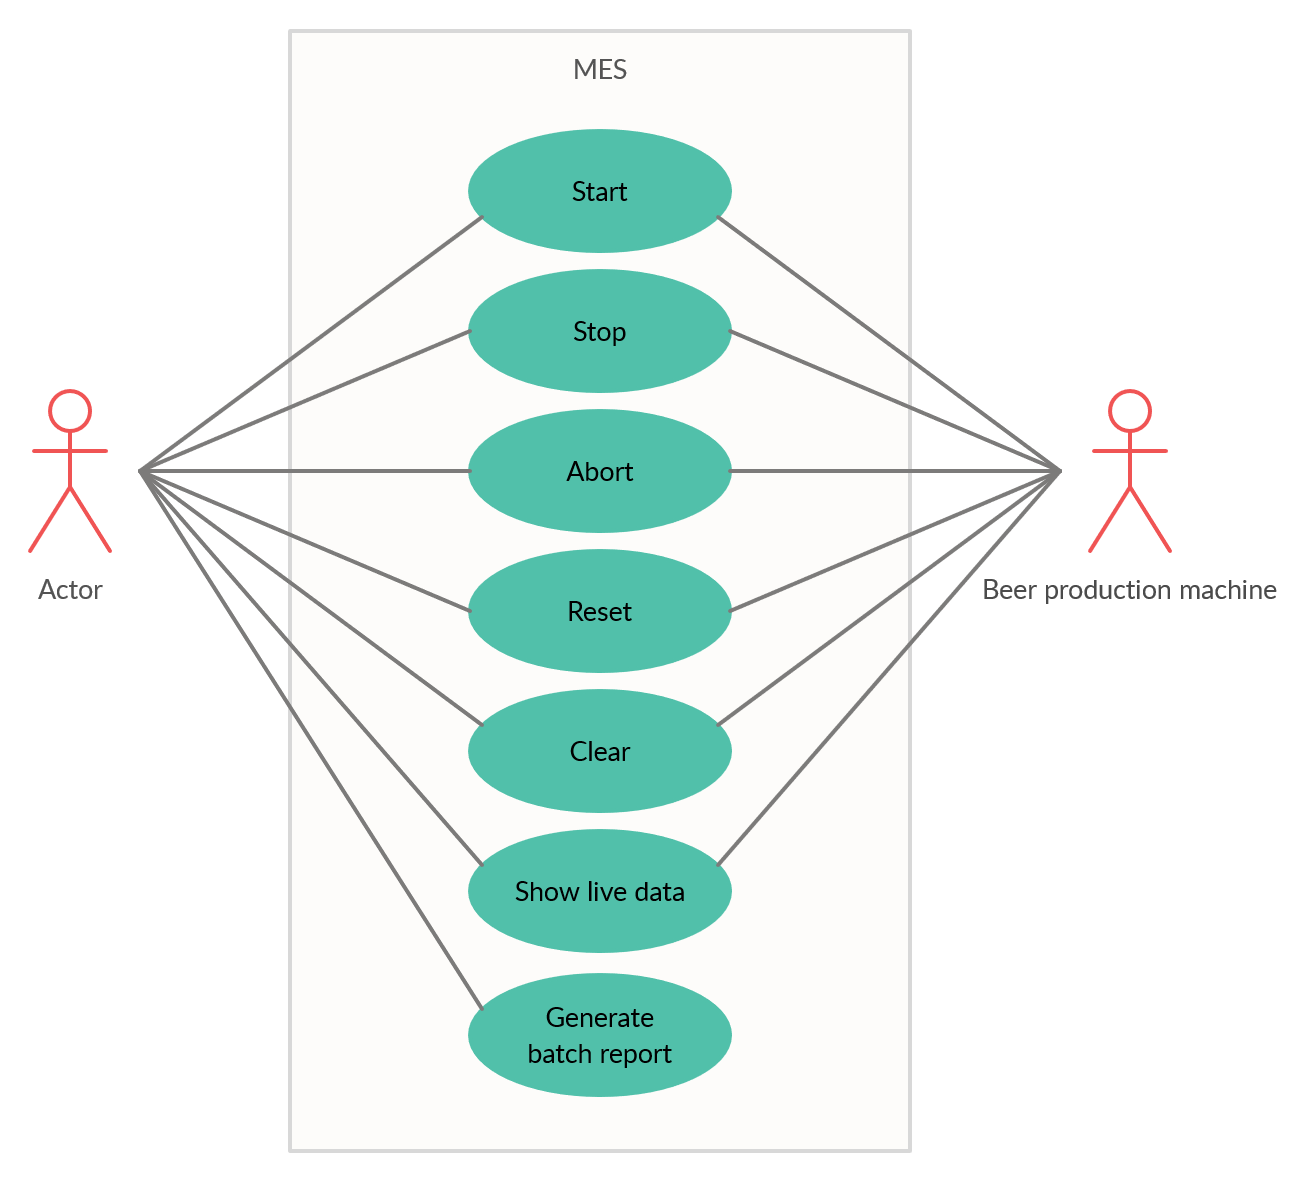
\includegraphics[scale=0.3]{images/ucdiagram.png}
	\caption{Use case diagram}
	\label{figure:ucdiagram} 
\end{figure}